\documentclass{exam}
\usepackage{../../commonheader}
\usepackage{outlines}

%%% CHANGE THESE %%%%%%%%%%%%%%%%%%%%%%%%%%%%%%%%%%%%%%%%%%%%%%%%%%%%%%%%%%%%%%
\discnumber{8}
\title{\textsc{Scheme}}
\date{October 31--November 4, 2022}
%%%%%%%%%%%%%%%%%%%%%%%%%%%%%%%%%%%%%%%%%%%%%%%%%%%%%%%%%%%%%%%%%%%%%%%%%%%%%%%

\begin{document}
\maketitle
\rule{\textwidth}{0.15em}
\fontsize{12}{15}\selectfont

\begin{guide}
\begin{blocksection}
\textbf{Recommended Timeline}
\begin{outline}[enumerate]
  \1 Scheme Mini-Lecture - 10 min
  \1 WWSD - 5 min
  \2 Could incorporate into minilecture
  \1 Hailstone - 8 min
  \2 Students should have seen this problem many times by now
  \2 Introduction to scheme with something they are familiar with
  \1 Scheme Lists Mini-Lecture - 6 min
  \1 Scheme List WWSD - 8 min
  \2 Could incorporate into minilecture
  \2 Drawing box \& pointer diagrams and making analogies to linked lists may be helpful
  \1 Decay - 8 min
  \2 introduces 'cond'
  \1 Waldo - 8 min
  \2 fun 'where's waldo' question haha
  \1 Challenge problem - if you have time
  \2 extension to Waldo, find the index waldo is at - if any
  \1 Exam Questions
  \2 completely optional, included as a reference so students can refer to these questions while studying
  \2 the best prep for exams is exam questions!
  \2 Sp22 Final Q11
  \3 requires 'append' function - might want to bring this up as a hint, if students haven't learned about this built-in function yet
  \3 constructing a scheme list
  \2 Su18 Final Q3b
  \3 drawing the box \& pointer diagrams of scheme lists
  \3 good to test and visualize understanding
\end{outline}
\end{blocksection}
\end{guide}

\section{Scheme}
\begin{guide}
\begin{blocksection}
\textbf{Teaching Tips}
\begin{outline}[enumerate]
    \1 To ease in Scheme, it can help to start by comparing and contrasting with Python
    \2 Have students write a basic function in Python (like an iterative countdown), then replicate it in Scheme
    \2 Have students list language features of Python (variable assignments, conditional statements, logic operators, etc.), and explain how Scheme implements those features
    \2 Make sure to give a disclaimer that while high level features may be analogous, the internals are different!
    \1 Scheme features break into three broad categories: Primitives, Call Expressions, and Special Forms (the latter two are called Compound Expressions)
    \2 Primitives evaluate to themselves (4 evaluates to 4, \#t to \#t, etc.)
    \2 Call Expressions begin with a function name and are followed by arguments- evaluate function name, evaluate arguments, and apply function to arguments
    \2 Special Forms begin with a keyword and are followed by subexpressions, which are evaluated in a way based on the specific keyword
    \1 Useful Links
    \2 \href{https://cs61a.org/articles/scheme-spec/}{Scheme Specification} (for overfiew, types, and special forms)
    \2 \href{https://cs61a.org/articles/scheme-builtins/}{Scheme Built-In Procedure Reference} (for built-in procedures)
\end{outline}
\end{blocksection}
\end{guide}

\subimport{../../topics/scheme/text/}{scheme-basics-overview.tex}
\begin{questions}
\newpage
\section{What Would Scheme Print?}
\subimport{../../topics/scheme/easy/wwsd/}{basics.tex}
\subimport{../../topics/scheme/easy/}{hailstone.tex}

\section{Scheme Lists}
\subimport{../../topics/scheme/text/}{scheme-lists-overview.tex}
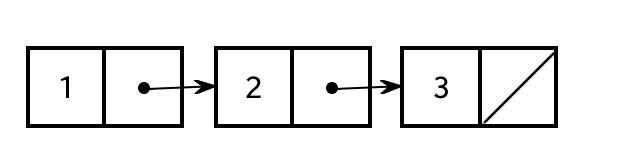
\includegraphics{../../topics/scheme/text/scheme_list.png}
\subimport{../../topics/scheme/text/}{special-forms.tex}
\newpage
\subimport{../../topics/scheme/easy/wwsd/}{lists_nodots.tex}
\subimport{../../topics/scheme/medium/}{binary-list.tex}
\subimport{../../topics/scheme/medium/}{is-prefix.tex}

\end{questions}

\end{document}